% Options for packages loaded elsewhere
\PassOptionsToPackage{unicode}{hyperref}
\PassOptionsToPackage{hyphens}{url}
\PassOptionsToPackage{dvipsnames,svgnames,x11names}{xcolor}
%
\documentclass[
sn-nature
]{sn-jnl}

\usepackage{amsmath,amssymb}
\usepackage{iftex}
\ifPDFTeX
  \usepackage[T1]{fontenc}
  \usepackage[utf8]{inputenc}
  \usepackage{textcomp} % provide euro and other symbols
\else % if luatex or xetex
  \usepackage{unicode-math}
  \defaultfontfeatures{Scale=MatchLowercase}
  \defaultfontfeatures[\rmfamily]{Ligatures=TeX,Scale=1}
\fi
\usepackage{lmodern}
\ifPDFTeX\else  
    % xetex/luatex font selection
\fi
% Use upquote if available, for straight quotes in verbatim environments
\IfFileExists{upquote.sty}{\usepackage{upquote}}{}
\IfFileExists{microtype.sty}{% use microtype if available
  \usepackage[]{microtype}
  \UseMicrotypeSet[protrusion]{basicmath} % disable protrusion for tt fonts
}{}
\makeatletter
\@ifundefined{KOMAClassName}{% if non-KOMA class
  \IfFileExists{parskip.sty}{%
    \usepackage{parskip}
  }{% else
    \setlength{\parindent}{0pt}
    \setlength{\parskip}{6pt plus 2pt minus 1pt}}
}{% if KOMA class
  \KOMAoptions{parskip=half}}
\makeatother
\usepackage{xcolor}
\setlength{\emergencystretch}{3em} % prevent overfull lines
\setcounter{secnumdepth}{5}
% Make \paragraph and \subparagraph free-standing
\makeatletter
\ifx\paragraph\undefined\else
  \let\oldparagraph\paragraph
  \renewcommand{\paragraph}{
    \@ifstar
      \xxxParagraphStar
      \xxxParagraphNoStar
  }
  \newcommand{\xxxParagraphStar}[1]{\oldparagraph*{#1}\mbox{}}
  \newcommand{\xxxParagraphNoStar}[1]{\oldparagraph{#1}\mbox{}}
\fi
\ifx\subparagraph\undefined\else
  \let\oldsubparagraph\subparagraph
  \renewcommand{\subparagraph}{
    \@ifstar
      \xxxSubParagraphStar
      \xxxSubParagraphNoStar
  }
  \newcommand{\xxxSubParagraphStar}[1]{\oldsubparagraph*{#1}\mbox{}}
  \newcommand{\xxxSubParagraphNoStar}[1]{\oldsubparagraph{#1}\mbox{}}
\fi
\makeatother


\providecommand{\tightlist}{%
  \setlength{\itemsep}{0pt}\setlength{\parskip}{0pt}}\usepackage{longtable,booktabs,array}
\usepackage{calc} % for calculating minipage widths
% Correct order of tables after \paragraph or \subparagraph
\usepackage{etoolbox}
\makeatletter
\patchcmd\longtable{\par}{\if@noskipsec\mbox{}\fi\par}{}{}
\makeatother
% Allow footnotes in longtable head/foot
\IfFileExists{footnotehyper.sty}{\usepackage{footnotehyper}}{\usepackage{footnote}}
\makesavenoteenv{longtable}
\usepackage{graphicx}
\makeatletter
\def\maxwidth{\ifdim\Gin@nat@width>\linewidth\linewidth\else\Gin@nat@width\fi}
\def\maxheight{\ifdim\Gin@nat@height>\textheight\textheight\else\Gin@nat@height\fi}
\makeatother
% Scale images if necessary, so that they will not overflow the page
% margins by default, and it is still possible to overwrite the defaults
% using explicit options in \includegraphics[width, height, ...]{}
\setkeys{Gin}{width=\maxwidth,height=\maxheight,keepaspectratio}
% Set default figure placement to htbp
\makeatletter
\def\fps@figure{htbp}
\makeatother
% definitions for citeproc citations
\NewDocumentCommand\citeproctext{}{}
\NewDocumentCommand\citeproc{mm}{%
  \begingroup\def\citeproctext{#2}\cite{#1}\endgroup}
\makeatletter
 % allow citations to break across lines
 \let\@cite@ofmt\@firstofone
 % avoid brackets around text for \cite:
 \def\@biblabel#1{}
 \def\@cite#1#2{{#1\if@tempswa , #2\fi}}
\makeatother
\newlength{\cslhangindent}
\setlength{\cslhangindent}{1.5em}
\newlength{\csllabelwidth}
\setlength{\csllabelwidth}{3em}
\newenvironment{CSLReferences}[2] % #1 hanging-indent, #2 entry-spacing
 {\begin{list}{}{%
  \setlength{\itemindent}{0pt}
  \setlength{\leftmargin}{0pt}
  \setlength{\parsep}{0pt}
  % turn on hanging indent if param 1 is 1
  \ifodd #1
   \setlength{\leftmargin}{\cslhangindent}
   \setlength{\itemindent}{-1\cslhangindent}
  \fi
  % set entry spacing
  \setlength{\itemsep}{#2\baselineskip}}}
 {\end{list}}
\usepackage{calc}
\newcommand{\CSLBlock}[1]{\hfill\break\parbox[t]{\linewidth}{\strut\ignorespaces#1\strut}}
\newcommand{\CSLLeftMargin}[1]{\parbox[t]{\csllabelwidth}{\strut#1\strut}}
\newcommand{\CSLRightInline}[1]{\parbox[t]{\linewidth - \csllabelwidth}{\strut#1\strut}}
\newcommand{\CSLIndent}[1]{\hspace{\cslhangindent}#1}

%%%% Standard Packages

\usepackage{graphicx}%
\usepackage{multirow}%
\usepackage{amsmath,amssymb,amsfonts}%
\usepackage{amsthm}%
\usepackage{mathrsfs}%
\usepackage[title]{appendix}%
\usepackage{xcolor}%
\usepackage{textcomp}%
\usepackage{manyfoot}%
\usepackage{booktabs}%
\usepackage{algorithm}%
\usepackage{algorithmicx}%
\usepackage{algpseudocode}%
\usepackage{listings}%

%%%%

\raggedbottom
\usepackage{booktabs}
\usepackage{longtable}
\usepackage{array}
\usepackage{multirow}
\usepackage{wrapfig}
\usepackage{float}
\usepackage{colortbl}
\usepackage{pdflscape}
\usepackage{tabu}
\usepackage{threeparttable}
\usepackage{threeparttablex}
\usepackage[normalem]{ulem}
\usepackage{makecell}
\usepackage{xcolor}
\makeatletter
\@ifpackageloaded{caption}{}{\usepackage{caption}}
\AtBeginDocument{%
\ifdefined\contentsname
  \renewcommand*\contentsname{Table of contents}
\else
  \newcommand\contentsname{Table of contents}
\fi
\ifdefined\listfigurename
  \renewcommand*\listfigurename{List of Figures}
\else
  \newcommand\listfigurename{List of Figures}
\fi
\ifdefined\listtablename
  \renewcommand*\listtablename{List of Tables}
\else
  \newcommand\listtablename{List of Tables}
\fi
\ifdefined\figurename
  \renewcommand*\figurename{Figure}
\else
  \newcommand\figurename{Figure}
\fi
\ifdefined\tablename
  \renewcommand*\tablename{Table}
\else
  \newcommand\tablename{Table}
\fi
}
\@ifpackageloaded{float}{}{\usepackage{float}}
\floatstyle{ruled}
\@ifundefined{c@chapter}{\newfloat{codelisting}{h}{lop}}{\newfloat{codelisting}{h}{lop}[chapter]}
\floatname{codelisting}{Listing}
\newcommand*\listoflistings{\listof{codelisting}{List of Listings}}
\makeatother
\makeatletter
\makeatother
\makeatletter
\@ifpackageloaded{caption}{}{\usepackage{caption}}
\@ifpackageloaded{subcaption}{}{\usepackage{subcaption}}
\makeatother
\ifLuaTeX
  \usepackage{selnolig}  % disable illegal ligatures
\fi
\usepackage{bookmark}

\IfFileExists{xurl.sty}{\usepackage{xurl}}{} % add URL line breaks if available
\urlstyle{same} % disable monospaced font for URLs
\hypersetup{
  pdftitle={ParaChiCSVO2},
  pdfauthor={Thomas Gavin Carmichael; Alexander Rauscher; Ruth E Grunau; Alexander Mark Weber},
  pdfkeywords={Quantitative Susceptbility
Mapping, Preterm, Newborn, Cerebral Venous Oxygen Saturation},
  colorlinks=true,
  linkcolor={blue},
  filecolor={Maroon},
  citecolor={Blue},
  urlcolor={Blue},
  pdfcreator={LaTeX via pandoc}}

\title[ParaChiCSVO2]{ParaChiCSVO2}

% author setup
\author[1,2]{\fnm{Thomas Gavin} \sur{Carmichael}}\email{tgcarmichael@outlook.com}\author[3]{\fnm{Alexander} \sur{Rauscher}}\email{rauscher@physics.ubc.ca}\author[2,3]{\fnm{Ruth E} \sur{Grunau}}\email{rgrunau@mail.ubc.ca}\author*[2,3]{\fnm{Alexander Mark} \sur{Weber}}\email{aweber@bcchr.ca}
% affil setup
\affil[1]{\orgdiv{Integrated Sciences}, \orgname{The University of
British Columbia}, \orgaddress{\street{2329 West
Mall}, \city{Vancouver}, \postcode{V6T 1Z4}, \country{Canada}}}
\affil[3]{\orgdiv{Pediatrics}, \orgname{The University of British
Columbia}, \orgaddress{\street{2329 West
Mall}, \city{Vancouver}, \postcode{V6T 1Z4}, \country{Canada}}}
\affil[2]{\orgdiv{BC Children's Hospital Research
Institute}, \orgname{The University of British
Columbia}, \orgaddress{\street{938 West 28th
Avenue}, \city{Vancouver}, \postcode{V5Z 4H4}, \country{Canada}}}

% abstract 

\abstract{\textbf{Background}: Quantitative susceptibility mapping (QSM)
is a magnetic resonance imaging (MRI) modality proposed to be a viable
method of measuring cerebral oxygenation in neonates given its
sensitivity to deoxyhemoglobin, a paramagnetic molecule. During QSM,
however, paramagnetic sources can be obscured by opposing diamagnetic
sources such as water and myelin. We sought to evaluate whether QSM
images alone, or an algorithm that attempts to isolate their
paramagnetic components, are more accurate in measuring oxygenation of
the major cerebral veins in a cohort of neonates born preterm.
Additionally, we aimed to determine whether a difference in oxygenation
existed between the major cerebral veins.

\textbf{Methods}: 19 neonates born preterm were scanned on a 3T research
MRI at term equivalent age. The protocol included a multi-echo
susceptibility-weighted imaging sequence. The acquired imaging data were
processed as QSM images to obtain the susceptibility values of the
superior sagittal sinus (SSS) and central cerebral veins (CCV). These
values were used to calculate the oxygen saturation (SvO2) of the SSS
and CCV. QSM images were subsequently processed to isolate their
paramagnetic components. SvO2 values of the SSS and CCV were calculated
again from the paramagnetic components.

\textbf{Results}: The mean SvO2 values of the SSS and CCV calculated
from QSM images were found to be 72.4\% (SD, 3.4\%) and 68.7\% (SD,
3.5\%), respectively. The mean SvO2 values calculated from paramagnetic
components were found to be 58.1\% (SD, 7.3\%) for the SSS and 57.7\%
(SD, 7.0\%) for the CCV.

\textbf{Conclusion}: SSS SvO2 values derived from paramagnetic
components agreed well with the existing literature and were closer than
the values derived from QSM, however, they displayed greater
variability. Although the CCV SvO2 data from QSM aligns more closely
with existing literature, it is important to note that the current
literature on this topic remains relatively limited in the CCV. Thus,
decomposing QSM images into paramagnetic components shows great promise
as a method for more accurately measuring cerebral oxygenation in
neonates but may require more research to improve precision. Notably, no
significant difference in oxygenation was observed between the CCV and
the SSS, contrasting with previous studies.}

% keywords
\keywords{Quantitative Susceptbility
Mapping,  Preterm,  Newborn,  Cerebral Venous Oxygen Saturation}

\begin{document}
\maketitle

\textsubscript{Source:
\href{https://WeberLab.github.io/Chisep_CSVO2_Manuscript/index.qmd.html}{Article
Notebook}}

\section{Introduction}\label{sec-intro}

\section{Methods}\label{sec-data-methods}

The study was approved by the Clinical Research Ethics Board at the
University of British Columbia and Children's \& Women's Hospital
(H21-00655) and written informed consent was obtained from the
parent/guardian for each infant.

\subsection{Study population}\label{study-population}

Participant data comes from a previous study. Participants consisted of
preterm neonates born between 25- and 31-weeks gestational age (GA) who
were admitted to the level III NICU at BC Women's Hospital. Recruitment
took place over a span of one year, from February 2021 to January 2022,
facilitated by a dedicated research nurse. Parents of eligible infants
were approached by the research nurse prior to discharge from the NICU
to explain the study objectives and seek their consent for
participation. Infants meeting the criteria for inclusion were scanned
for the study if they had already been discharged from the NICU, were in
stable condition, and had reached a term equivalent age of 37 to 44
weeks GA. However, certain exclusion criteria were applied to ensure the
homogeneity and integrity of the study sample. Infants were excluded if
there was clinical evidence of a congenital malformation or syndrome, a
TORCH infection, or ultrasound evidence of large parenchymal hemorrhagic
infarction (\textgreater2 cm, Grade 4 intraventricular hemorrhage).

\subsection{Image acquisition}\label{image-acquisition}

MR imaging was performed on a 3.0 Tesla General Electric Discovery MR750
scanner (scanner software version DV26.0\_R03) equipped with a SREE
Medical Systems single-channel neonatal head coil (Table~\ref{tbl-mri}).
The scans were conducted at the BC Children's MRI Research Facility.
Prior to the scanning procedure, subjects were carefully prepared by a
research nurse. Swaddling and feeding were used to ensure the comfort
and cooperation of the subjects during the scan. Importantly, no
sedatives or invasive markers were utilized throughout the procedure.
Subjects were placed within a specially designed SREE Medical Systems
MRI compatible incubator, which facilitated both safety and motion
minimization. Molded foam was strategically positioned around the head
and body within the incubator to further restrict subject movement. To
protect against potential hearing damage, ear plugs were employed during
the scanning process. Additionally, a pulse oximeter was affixed to the
subject's foot to monitor arterial oxygen saturation and heart rate
throughout the scan.

\begin{longtable}[]{@{}
  >{\raggedright\arraybackslash}p{(\columnwidth - 8\tabcolsep) * \real{0.1918}}
  >{\raggedright\arraybackslash}p{(\columnwidth - 8\tabcolsep) * \real{0.1918}}
  >{\raggedright\arraybackslash}p{(\columnwidth - 8\tabcolsep) * \real{0.1918}}
  >{\raggedright\arraybackslash}p{(\columnwidth - 8\tabcolsep) * \real{0.2329}}
  >{\raggedright\arraybackslash}p{(\columnwidth - 8\tabcolsep) * \real{0.1918}}@{}}
\caption{Technical parameters for MR imaging
protocol.}\label{tbl-mri}\tabularnewline
\toprule\noalign{}
\begin{minipage}[b]{\linewidth}\raggedright
\end{minipage} & \begin{minipage}[b]{\linewidth}\raggedright
T1w
\end{minipage} & \begin{minipage}[b]{\linewidth}\raggedright
T2w
\end{minipage} & \begin{minipage}[b]{\linewidth}\raggedright
pcASL
\end{minipage} & \begin{minipage}[b]{\linewidth}\raggedright
SWI
\end{minipage} \\
\midrule\noalign{}
\endfirsthead
\toprule\noalign{}
\begin{minipage}[b]{\linewidth}\raggedright
\end{minipage} & \begin{minipage}[b]{\linewidth}\raggedright
T1w
\end{minipage} & \begin{minipage}[b]{\linewidth}\raggedright
T2w
\end{minipage} & \begin{minipage}[b]{\linewidth}\raggedright
pcASL
\end{minipage} & \begin{minipage}[b]{\linewidth}\raggedright
SWI
\end{minipage} \\
\midrule\noalign{}
\endhead
\bottomrule\noalign{}
\endlastfoot
Sequence & 3D FSPGR & 3D CUBE & Multi-shot 3D fast spin-echo & 3D
spoiled GRE flow-compensated \\
Phase-encoding direction & Coronal & Sagittal & Axial & Axial \\
TR (ms) & 7.74 & 2,300 & 4,680 & 30.9 \\
TE (ms) & 2.97 & 66.29 & 10.55 & 5.24 \\
Flip angle & 12\(^{\circ}\) & 90\(^{\circ}\) & 111\(^{\circ}\) &
20\(^{\circ}\) \\
FOV (cm) & 20 & 20 & 24 & 25 \\
Acquisition Matrix & 512 x 512 & 256 x 256 & 128 x 128 & 256 x 256 \\
In-plane resolution (mm) & 0.39 x 0.39 & 0.78 x 0.78 & 1.875 x 1.875 &
0.977 x 0.977 \\
Slice thickness (mm) & 1 & 1 & 4 & 2, reconstructed to 1 mm with zero
filling (ZIP2) \\
Number of slices & 126 & 106 & 50 & 92 \\
Additional parameters & n/a & n/a & 1,450 ms label period; 2,025 ms
pulse lable; 24 control-label pairs & n/a \\
Scan duration & 4 min 39 s & 5 min 1 s & 5 min 26 s & 5 min 29 s \\
\end{longtable}

The MRI scan protocol comprised several sequences, including a
T1-weighted scan, a T2-weighted scan, a pseudo-continuous arterial spin
labeling (ASL) scan, a multi-echo susceptibility-weighted imaging scan,
and a diffusion-weighted imaging (DWI) spin-echo echo planar imaging
(EPI) sequence.

\begin{figure}[H]

\centering{

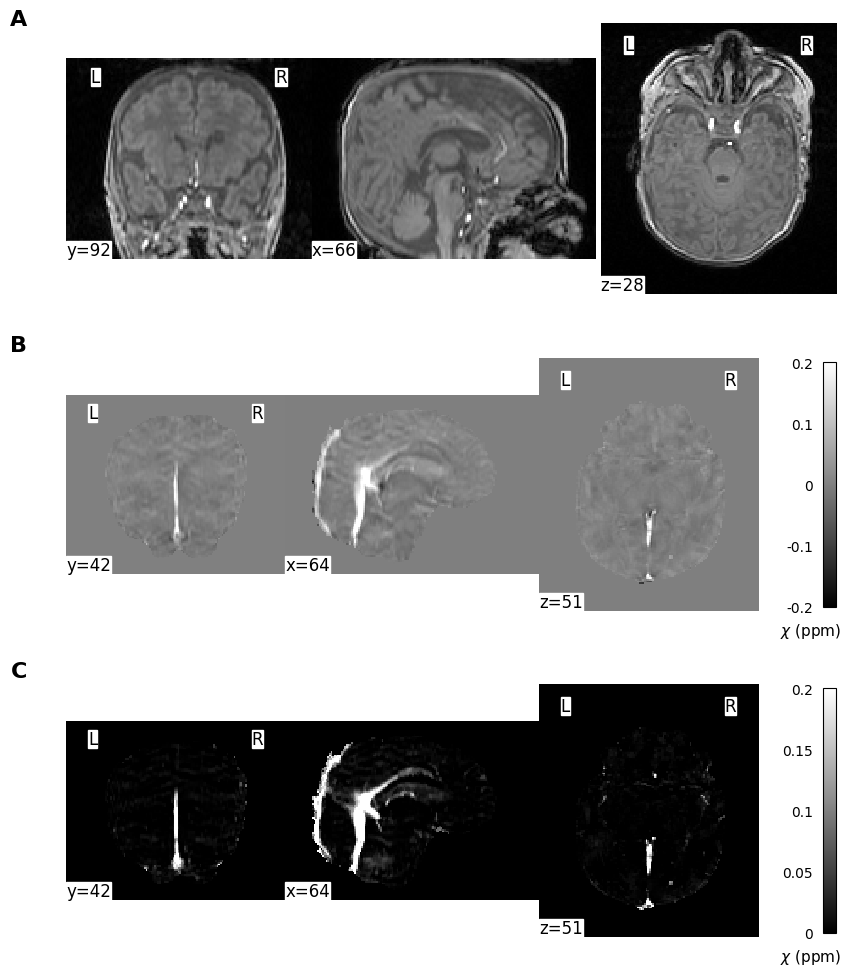
\includegraphics{index_files/figure-latex/notebooks-Figures-fig-sample-output-1.png}

}

\caption{\label{fig-sample}Sample images}

\end{figure}%

\textsubscript{Source:
\href{https://WeberLab.github.io/Chisep_CSVO2_Manuscript/notebooks/Figures.ipynb.html\#cell-fig-sample}{Python
Figures}}

See Figure~\ref{fig-graph}

\begin{figure}[H]

\centering{

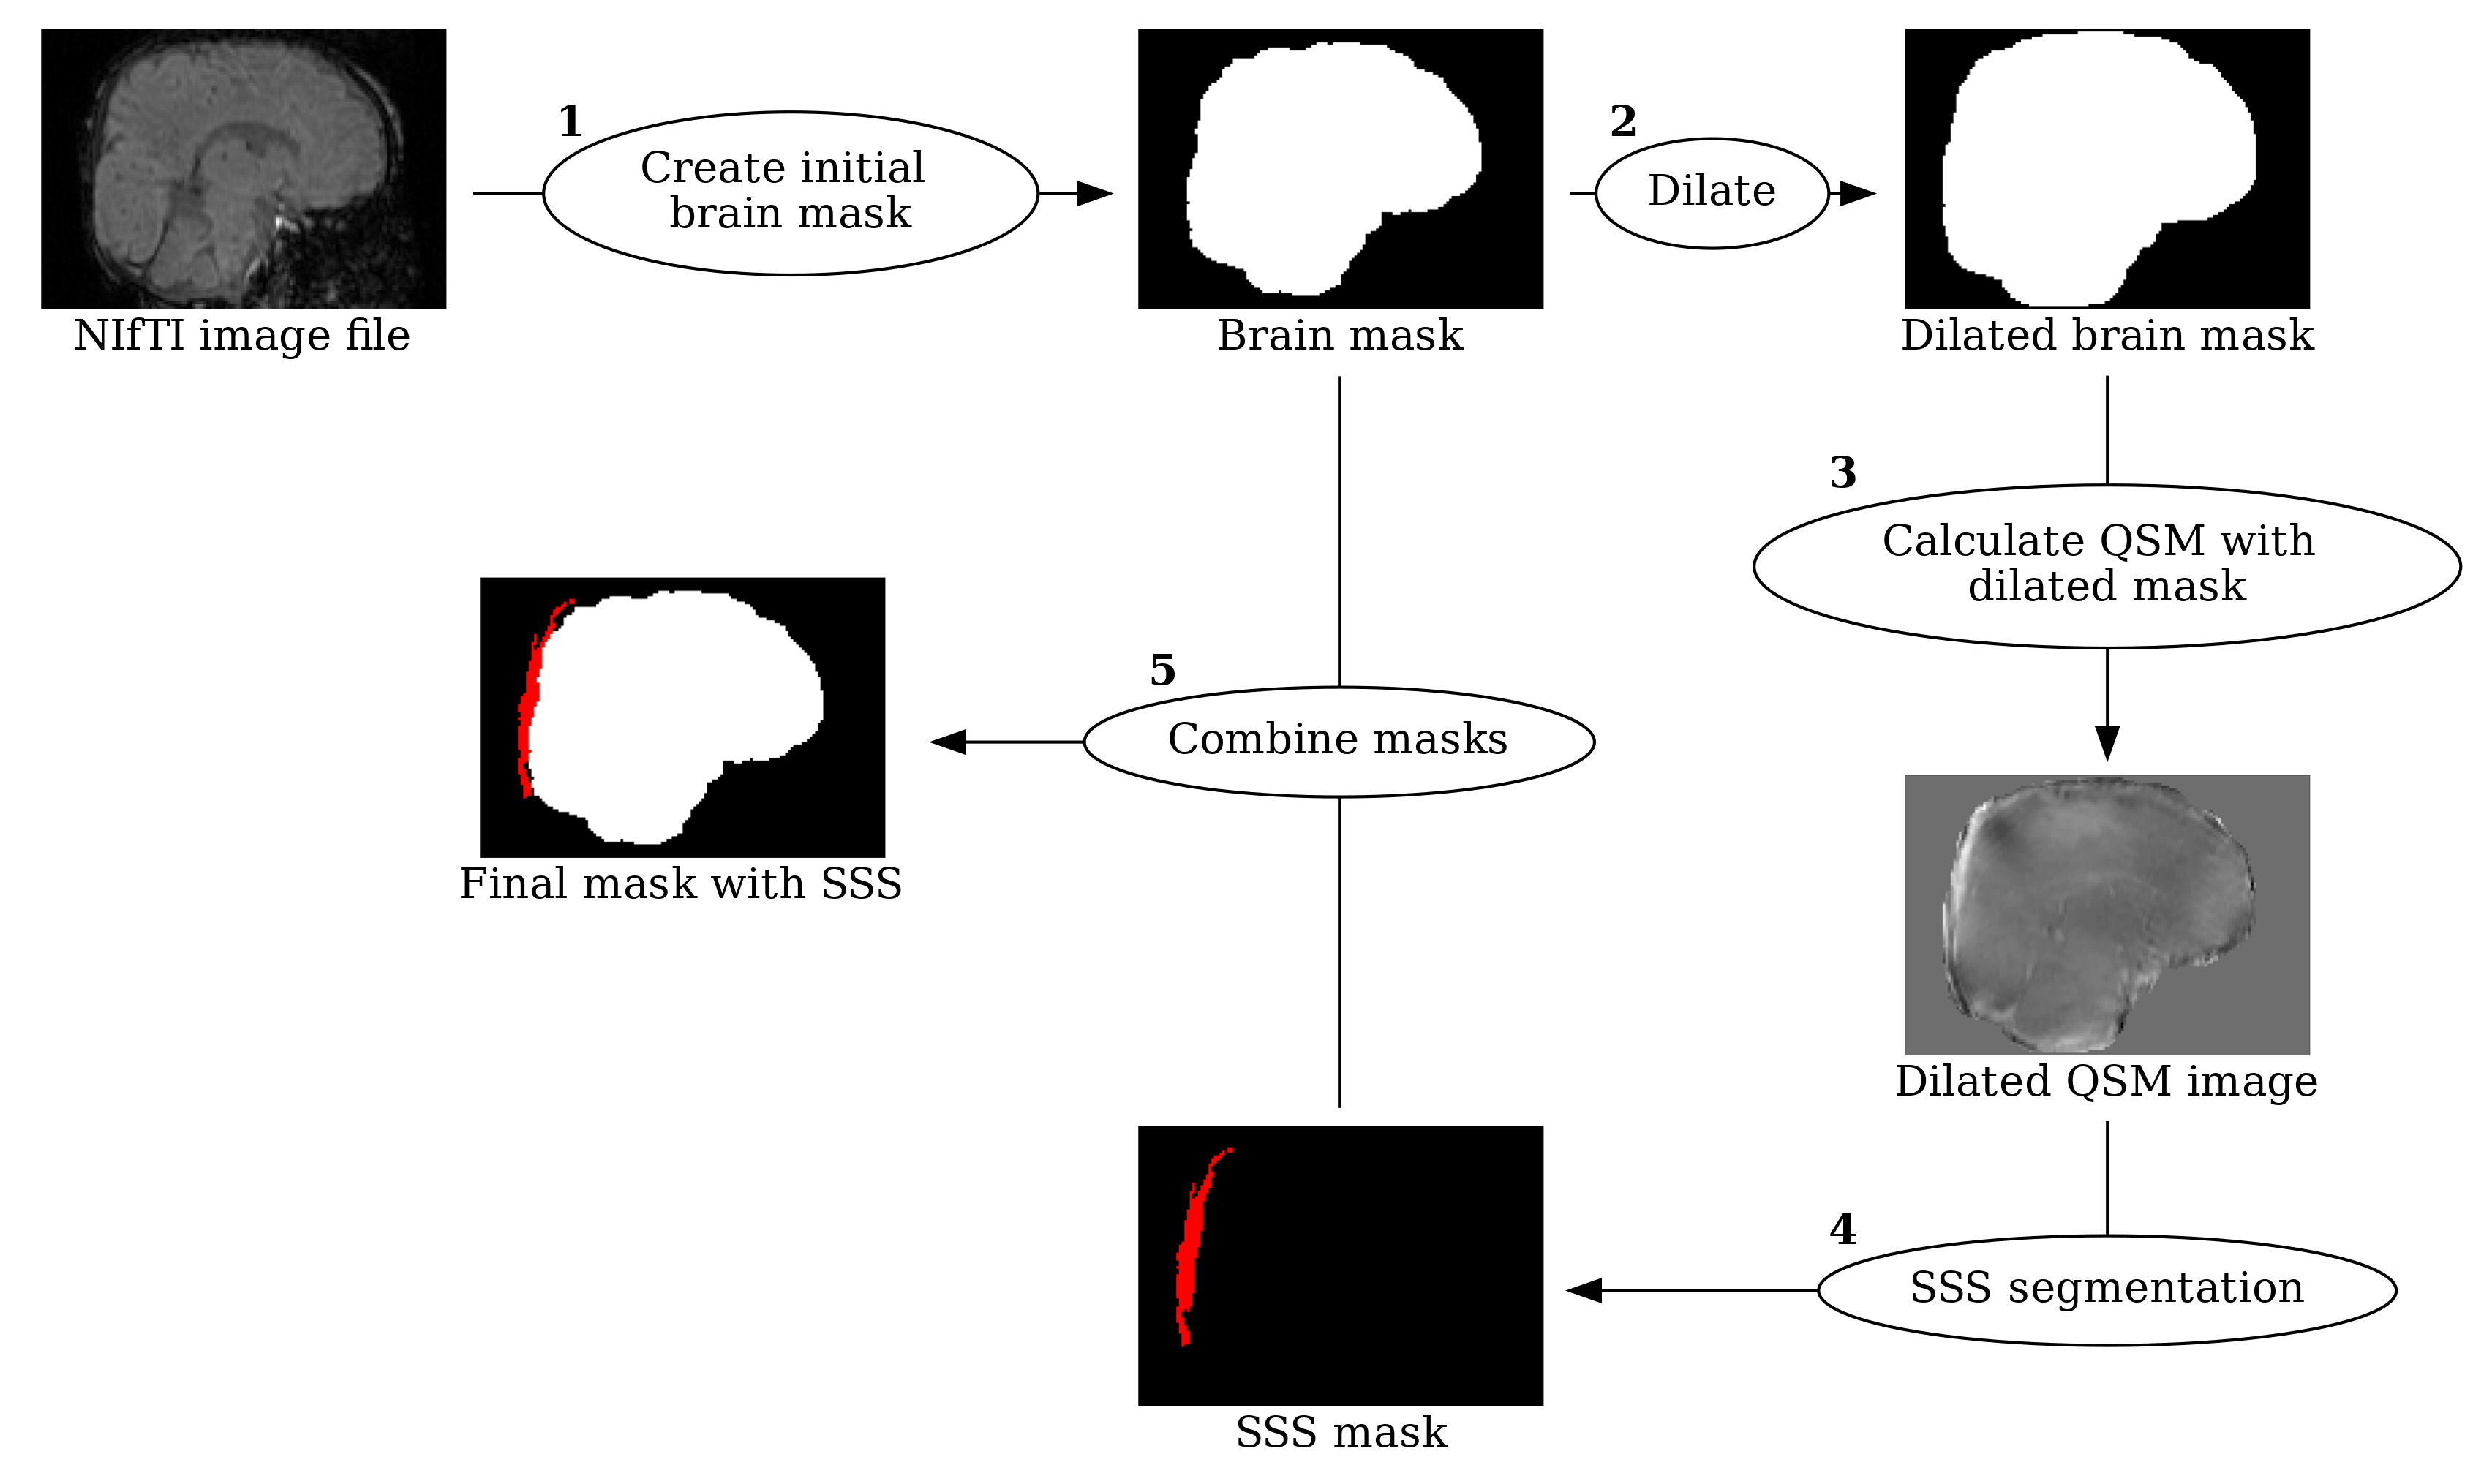
\includegraphics{index_files/figure-latex/notebooks-Figures-fig-graph-output-1.png}

}

\caption{\label{fig-graph}A graph of the methods to create a mask}

\end{figure}%

\textsubscript{Source:
\href{https://WeberLab.github.io/Chisep_CSVO2_Manuscript/notebooks/Figures.ipynb.html\#cell-fig-graph}{Python
Figures}}

\section{Results}\label{sec-results}

(Ahmed et al. 2023)

\section{Conclusion}\label{sec-conclusion}

\section*{References}\label{references}
\addcontentsline{toc}{section}{References}

\phantomsection\label{refs}
\begin{CSLReferences}{1}{0}
\bibitem[\citeproctext]{ref-ahmedDiamagneticComponentMap2023a}
Ahmed, Maruf, Jingjia Chen, Arvin Arani, Matthew L. Senjem, Petrice M.
Cogswell, Clifford R. Jack, and Chunlei Liu. 2023. {``The Diamagnetic
Component Map from Quantitative Susceptibility Mapping ({QSM}) Source
Separation Reveals Pathological Alteration in {Alzheimer}'s
Disease-Driven Neurodegeneration.''} \emph{NeuroImage} 280 (October):
120357. \url{https://doi.org/10.1016/j.neuroimage.2023.120357}.

\end{CSLReferences}



\end{document}
